\chapter{Implementació i Proves}
\label{cap:11}

Durant aquesta implementació, s'enumeraran els diferents passos seguits per dur a terme el projecte. Aquests passos es citaran en l'idioma en què han estat utilitzats durant la pràctica, de manera que és possible que apareguin en diferents idiomes (principalment anglès i castellà) en reproduir aquests exemples.

\section{Obtenció de la màquina al GCP}

Donat que ja es disposava del portàtil, el primer pas durant la implementació va ser la creació d'una màquina que s'utilitzaria al \textit{Google Cloud Platform}.

\subsection{Creació d'un compte de Google}

El primer pas és tenir un compte de Google, que sol tenir un gran percentatge de la població, ja que és el compte que permet l'accés a aplicacions populars com Gmail i Drive. A més, s'utilitza per augmentar les funcionalitats d'altres serveis com el sistema operatiu Android o la pàgina web YouTube. La creació d'un compte de Gmail és molt senzilla. Cal anar a \textit{gmail.com} i seguir les següents instruccions, clicant el botó \textit{Siguiente} després de cada pas: \begin{enumerate} \item Clicar a \textit{Crear cuenta} i escriure el nom a la casella corresponent. \item Posar la data de naixement i el sexe. \item Escollir una adreça de Gmail, que serà l'identificador amb el qual es relacionarà el compte. \item Escollir la contrasenya i repetir-la, que serà la clau per entrar al compte juntament amb l'identificador. \item Escriure un número de telèfon accessible per verificar el compte mitjançant un SMS. \item Introduir el codi de verificació que es rebrà al telèfon per part de Google a l'aplicació de SMS. \end{enumerate}

Un cop es tingui un compte de Google, ja es pot procedir al següent apartat per crear el compte de \textit{Google Cloud} a partir del compte de Google.

\subsection{Creació d'un compte de GCP a partir del compte de Google}

Per seguir aquesta secció, es donarà per suposat que la sessió del compte de Google està iniciada. Per començar, caldrà anar a \textit{cloud.google.com} i clicar a \textit{Get started for free}. Posteriorment, caldrà seguir les següents instruccions:

\begin{enumerate} \item Escollir el compte de Google que s'utilitzarà i seleccionar el país. Després, prémer \textit{Agree \& Continue}. \item Escollir el tipus de compte (\textit{Individual} en aquest cas) i emplenar els detalls personals. \item Emplenar els detalls de la targeta de crèdit on es cobraran els costos del compte. Caldrà introduir les dades privades i confirmar amb l'aplicació del banc. \item Finalment, prémer \textit{START FREE}. \end{enumerate}

\subsection{Instanciació de la màquina}

Per instanciar una màquina, cal anar primer a la pàgina web \textit{console.cloud.google.com}. Allà es trobarà l'opció \textit{Create a VM}. En clicar-hi, el següent pas és crear un projecte per a aquest entorn en particular, que consisteix a crear un entorn que pot tenir moltes màquines, taulers de dades personalitzats, etc.

És una bona pràctica crear un projecte per no barrejar màquines de diferents assumptes i així tenir una millor organització. Per crear un nou projecte, haurem de clicar al selector que està al costat de la icona de Google Cloud a la part superior esquerra. Amb això s'obrirà un desplegable a la mateixa pestanya, on es podrà clicar al botó \textit{NEW PROJECT}. Llavors s'obrirà l'opció de posar un nom a aquest nou projecte i triar una organització. Aquesta opció és utilitzada quan el compte forma part d'una empresa, i per tant, tot el que costi la infraestructura d'aquest projecte estarà pagat per una organització de l'empresa (o podria ser tota l'empresa part d'una sola organització si aquesta és molt petita). En aquest cas, no es seleccionarà cap organització, ja que es pagarà amb els crèdits gratuïts que ofereix GCP al principi, i posteriorment amb una targeta de crèdit quan aquests s'esgotin.

Ara que ja tenim el nou projecte creat, el podem seleccionar i procedir a crear la màquina. Les característiques de la màquina ja estan especificades a la \autoref{Tab:MaquinaServidorNuvul}, amb l'addició de les següents característiques que s'han triat:

\begin{itemize} \item La Regió és europe-west1 (Bèlgica), ja que és força econòmica. \item La Zona és europe-west1-b. \item El Model d'aprovisionament és Estàndard, per tant, la màquina sempre estarà activa si està encesa. \item El Sistema operatiu és Ubuntu 22.04 LTS. \item Al Tallafocs es permet tràfic HTTP i HTTPS, que s'utilitzarà per interactuar amb el servidor. \item La Interfície de xarxa és la \textit{default}, que tenen tots els comptes nous per defecte. \end{itemize}

Amb això, se'ns crearà la màquina al cap de pocs minuts, i podrem interactuar-hi amb el protocol \textit{ssh}, un protocol popular per controlar una màquina remota amb línia de comandes.

\newpage
\section{Instal·lació del servidor a les màquines}

El procediment per instal·lar els servidors a les dues màquines és molt similar, ja que ambdues són màquines de tipus \textit{linux}, el tipus més popular per a màquines dedicades a ser servidors gràcies al caràcter obert i la gran quantitat d'eines disponibles per a usuaris experimentats. A les dues màquines s'instal·larà \textit{Docker Engine} i \textit{Docker Compose}, que són necessaris perquè el servidor pugui funcionar. A continuació, es descarregarà el servidor mitjançant git, es navegarà a la carpeta corresponent i s'executarà amb la comanda \textit{Make}, una comanda que executa l'arxiu local anomenat \textit{Makefile} amb els arguments que se li passin, la qual és una manera popular de gestionar múltiples contenidors amb \textit{Docker Compose}.

\subsection{Instal·lació a la màquina del núvol}

La instal·lació a Ubuntu consisteix a actualitzar el repositori de paquets, instal·lar paquets que permeten la comunicació per HTTPS amb els seus certificats necessaris, afegir els paquets oficials de Docker a la llista de repositoris que volem que la nostra màquina utilitzi a l'hora de descarregar paquets, instal·lar Docker i Docker Compose i, finalment, descarregar el repositori amb git, navegar a la carpeta corresponent i executar el servidor.

\begin{lstlisting}[language=bash, caption=Instruccions per instal·lar el servidor al núvol]
 sudo apt update
 sudo apt install apt-transport-https ca-certificates curl software-properties-common
 curl -fsSL https://download.docker.com/linux/ubuntu/gpg | sudo apt-key add -
 sudo apt install docker
 sudo apt install docker-compose
 git clone https://github.com/make-apis-fun/make-apis-fun.git
 cd make-apis-fun/games/clue-api/
 sudo make up
\end{lstlisting}


\subsection{Instal·lació a la màquina local}

El portàtil que s'utilitza com a local, utilitza el sistema operatiu \textit{Arch Linux}, un sistema operatiu molt minimalista al qual l'usuari ha de construir a la seva mesura mitjançant línia de comandes fins a arribar a tenir l'experiència habitual d'una interfície d'escriptori amb els seus programes amb interfície gràfica.

A causa d'això, molts programes com \textit{Docker}, \textit{Docker Compose} i \textit{Git} han estat instal·lats juntament amb molts altres programes habituals a l'hora de fer ús del portàtil com a desenvolupador. Per això, la instal·lació ha consistit únicament en el següent:

\begin{lstlisting}[language=bash, caption=Instruccions per instal·lar el servidor al local]
 git clone https://github.com/make-apis-fun/make-apis-fun.git
 cd make-apis-fun/games/clue-api/
 sudo make up
\end{lstlisting}

En cas que, en intentar reproduir, no estiguin instal·lats els 3 paquets necessaris, es poden instal·lar fàcilment amb el gestor de paquets oficial de \textit{Arch Linux}, anomenat \textit{Pacman}. Primer, actualitzarem el repositori de paquets i, posteriorment, instal·lem els paquets que ens interessen. Finalment, farem que \textit{Docker Engine} s'encengui automàticament cada cop que s'encengui la màquina mitjançant el servei \textit{systemd} que ve instal·lat amb el paquet de Docker.
\begin{lstlisting}[language=bash, caption=Instruccions per els prerequisits al local]
 sudo pacman -Syu
 sudo pacman -S git docker docker-compose
 sudo systemctl start docker.service
 sudo systemctl enable docker.service
\end{lstlisting}

\subsection{Comprovació del funcionament}

Per comprovar que funcionen, es pot utilitzar l'eina \textit{curl}, que permet rebre el contingut d'un servidor web. La seva utilització és molt senzilla en aquest cas; a més, està preinstal·lada al sistema operatiu \textit{Ubuntu}, i també es va instal·lar en algun moment en el \textit{Arch Linux}. Només cal passar com a argument la direcció IP del servidor i el port al qual es vol fer la consulta. En aquest cas, la direcció serà la màquina en si mateixa, referida a Linux amb l'àlies de \textit{localhost}, i el port per defecte del nostre servidor, que és 8085.

\begin{lstlisting}[language=bash, caption=Petició localhost al servidor]
    curl localhost:8085
\end{lstlisting}

Al fer aquesta petició, immediatament rebem \textit{Welcome to the Clue API. Let's start creating a game. We encourage you to read the documentation about how to play}, que ens confirma que el servidor està actiu i que es pot connectar des de la mateixa màquina.

\newpage \section{Obrir l'accés dels servidors a internet}

Per tal que els servidors siguin accessibles des d'internet, cal tenir en compte dos factors: Cal verificar si altres màquines de la nostra xarxa poden accedir als ports de la màquina, i si màquines d'altres xarxes poden trobar el servidor mitjançant una IP i un port públics.

La resposta sol dependre de si la màquina té un tallafocs actiu o no. Tots els sistemes derivats de Linux disposen d'un tallafocs actiu, que funciona com a part del nucli de Linux, ja que sol ser essencial per a la seguretat d'un sistema operatiu, i, per tant, bloqueja qualsevol accés als ports per part d'una màquina forana. Per permetre l'accés a algun port de la màquina des de la xarxa, cal instal·lar un paquet que gestioni el tallafocs, que en aquest cas és \textit{ufw}, i especificar a quin port volem permetre l'accés des de la xarxa.

La segona part és on es veu molt més la diferència entre la xarxa de l'ordinador local i la xarxa de l'ordinador al núvol. En el cas de l'ordinador local, s'haurà d'accedir al router i configurar manualment l'entrada a la taula de traducció NAT, de manera que qualsevol paquet que arribi al router a un port específic s'enviï al nostre servidor. Per altra banda, a \textit{Google Cloud} no cal interactuar amb cap router físic, sinó que s'haurà de fer mitjançant les eines que Google posa a disposició al GCP.

\subsection{Obrir l'accés del servidor local a internet}

El primer pas és instal·lar i activar el tallafocs a la màquina, fer que aquest s'encengui automàticament cada cop que s'iniciï l'ordinador i, després, afegir la norma que permeti l'accés a les màquines foranes al port que està utilitzant Docker:

\begin{lstlisting}[language=bash, caption=Instalació del tallafocs al servidor local]
    sudo pacman -S ufw
    sudo ufw enable
    sudo systemctl start ufw.service
    sudo systemctl enable ufw.service
    sudo ufw allow 8085
\end{lstlisting}

A continuació, cal afegir el nostre servidor al router mitjançant el procés anomenat \textit{Redirecció de ports}. En aquest cas, el router és un model de la marca \textit{ZTE} de la companyia de telecomunicacions \textit{Digi}, del qual es disposa d'un manual a internet sobre com accedir-hi i obrir els ports. La majoria de companyies ofereixen aquesta informació a internet, així que per reproduir aquest pas es recomana buscar el model del router que es tingui i seguir les instruccions. En aquest cas en particular, s'ha de seguir la següent seqüència d'instruccions:

\label{subsec:PortForwardingLocal}

\begin{enumerate} \item Anar a \textit{192.168.1.1}, que sol ser la direcció local de la gran majoria de routers. \item Introduir el nom d'usuari i la contrasenya. Si mai s'ha canviat, es podrà trobar al manual del router o de la companyia. \item Clicar a \textit{Internet}. \item Clicar a \textit{Security}. \item Clicar a \textit{Port Forwarding}. \item Afegir un nou \textit{Item}. \item Escriure la \textit{MAC} o \textit{IP} de la màquina dins la xarxa local on serà el servidor. \item Escriure el port pel qual arribaran les peticions al router. \item Escriure a quin port de la màquina s'hauran d'enviar les peticions. \item Escriure quines \textit{IPs} d'internet podran accedir al nostre servidor. En el nostre cas, triem \textit{0.0.0.0}. \end{enumerate}

Amb això, en condicions normals ja es podria accedir al servidor des d'internet. No obstant això, es va descobrir que el router local estava sota un \textit{NAT massiu}, de manera que l'única forma de fer accessible el servidor a internet era contactar amb la companyia \textit{Digi}. El suport tècnic va confirmar que no hi havia cap error que impedís l'obertura de ports, però van indicar que, per tal que funcionés correctament, calia contractar una funcionalitat anomenada \textit{Conexión Plus}, que permet sortir del \textit{NAT massiu} i obtenir una IP estàtica. Aquesta funcionalitat té un cost de 1€/mes, que es va contractar per poder dur a terme aquest projecte.

\subsection{Obrir l'accés del servidor al núvol a internet}

La instal·lació i execució del tallafocs és gairebé idèntica a la del servidor de la màquina local, amb l'excepció que aquest cop utilitzarem el gestor de paquets d'Ubuntu, \textit{apt}:

\begin{lstlisting}[language=bash, caption=Instalació del tallafocs al servidor del núvol]
    sudo apt update
    sudo apt install ufw
    sudo ufw enable
    sudo systemctl start ufw.service
    sudo systemctl enable ufw.service
    sudo ufw allow 8085
\end{lstlisting}

\label{subsec:PortForwardingCloud}
D'altra banda, com que la màquina està al núvol, no es pot accedir directament al seu router, sinó que tot es gestiona des del portal \textit{console.cloud.google.com/net-security/firewall-manager/firewall-policies/}. A dalt, tindrem l'opció de crear una \textit{firewall rule}, que haurem de configurar amb informació similar a la de la subsecció de la màquina local:

\begin{enumerate} \item Clicar el botó \textit{CREATE FIREWALL RULE}. \item Escriure un nom per a la norma. \item Triar la \textit{Network} on es trobi la nostra màquina, \textit{default} en aquest cas. \item Seleccionar \textit{All instances in the network} a la categoria de \textit{Targets}. \item A sota de \textit{Source filter}, escriure \textit{0.0.0.0/0}, és a dir, permetre a tots els dispositius de fora la xarxa accedir al servidor. \item A \textit{Specified protocols and ports}, escollir \textit{TCP} i escriure a sota \textit{8085}, el port de la nostra màquina. \end{enumerate}

\newpage \section{Creant l'entorn per a la Màquina Client} 
\label{màquina client}
\subsection{Instal·lació de k6 i Chocolatey}

La manera més fàcil d'instal·lar l'eina k6 és instal·lant abans \textit{Chocolatey}, un gestor de paquets molt popular entre desenvolupadors a \textit{Windows}. Això es pot fer obrint la consola \textit{Powershell} com a administrador i executant la següent comanda:

\begin{lstlisting}[language=bash, caption=Instal·lació de \textit{Chocolatey}]
    Set-ExecutionPolicy Bypass -Scope Process -Force; [System.Net.ServicePointManager]::SecurityProtocol = [System.Net.ServicePointManager]::SecurityProtocol -bor 3072; iex ((New-Object System.Net.WebClient).DownloadString('https://community.chocolatey.org/install.ps1'))
\end{lstlisting}

A la mateixa consola es pot executar la següent comanda per a la instal·lació de \textit{k6}:

\begin{lstlisting}[language=bash, caption=Instal·lació de k6 mediant \textit{Chocolatey}]
    choco install k6 -confirm
\end{lstlisting}

\subsection{Descarrega dels scripts}

Per a la descarrega dels scripts de k6 per a aquest projecte, es farà servir l'eina \textit{Git} per a descarregar el projecte amb el codi allotjat a \textit{Github}. Fem servir el mateix mètode que anteriorment per instal·lar-ho amb \textit{Chocolatey}. Posteriorment, descarreguem el projecte a la nostra màquina.alar-ho amb \textit{Chocolatey}. Posteriorment descarreguem el projecte a la nostra maquina.

\begin{lstlisting}[language=bash, caption=Instal·lació de git i clonació del projecte]
    choco install git
    git clone https://github.com/CRiSTiK24/k6scripts.git
\end{lstlisting}

Això crearà una carpeta idèntica a la que està penjada a la web de \textit{Github}, cosa que ens permetrà modificar-la i enviar canvis a \textit{Github} de manera fàcil. A l'inrevés, també podrem absorbir qualsevol canvi fet a \textit{Github} al nostre projecte.

En el projecte es trobarà el següent codi anomenat \textit{script.js}, que serà el test de càrrega utilitzat. A continuació es pot veure el test, que consisteix a importar un arxiu amb les IPs dels dos servidors i escollir-ne un segons el número que es passi per paràmetre. També depèn del paràmetre la quantitat de màquines que volem tenir al primer minut d'execució i al segon. Al tercer minut d'execució, volem que el nombre de \textit{Virtual Users} arribi a 0. En el programa es fan diverses crides; la primera i la tercera són crides que no canviaran l'estat del servidor, mentre que el segon i el quart sí que ho faran. Al test es controlarà que les crides hagin estat satisfactòries i que el 90\% de les crides es resolguin en menys de 500 milisegons. Finalment es ferà que el \textit{Virtual User} es pari 5 segons al haver fet i comprovat les crides, avans de simular un usuari nou conectant-se.

\label{codi:testDeCarrega}
\newpage
\lstinputlisting[language=JavaScript, caption=Test de càrrega]{Codi/script.js}

\newpage
\section{Instal·lació de Netdata a les Màquines-Servidors}

\textit{Netdata}, el programa que es ferà servir per visualitzar remotament les analítiques desde internet, necesitarà en essencia els mateixos pasos que s'han seguit per instalar el servidor: Instalar el paquet, permetre la conexió al tallafocs i fer la redirecció de ports. \cite{noauthor_netdata_nodate}

\subsection{Instal·lació de Netdata a la màquina local}

\begin{lstlisting}[language=bash, caption=Instal·lació de netdata al local]
 sudo pacman -S git netdata
 sudo systemctl start netdata.service
 sudo systemctl enable netdata.service
 sudo ufw allow 19999
\end{lstlisting}

Amb això es pot consultar desde el  portatil mateix que \textit{localhost:19999} tindrà la webapp activa. Finalment s'haurà d'accedir al router de la mateixa manera que s'ha fet per el servidor del joc senzill a l'apartat \ref{subsec:PortForwardingLocal}, i aquest cop obrir el port 19999, que és el que utilitza per defecte netdata, en comptes del 8085.

\subsection{Instal·lació de Netdata a la màquina al núvol}

Per instalar \textit{Netdata} a \textit{Ubuntu}, al contrari que a \textit{Arch Linux} on es sol recomenar sempre utilitzar \textit{pacman} per a tots els paquets, s'utilitzarà la recomenació de la pàgina web de \textit{Netdata}, on es diu de descarregar un \textit{Shell script} amb textit{curl} que gestionarà la instalació. Caldrà escriure intermitentmet \textit{Y} per a confirmar les comandes que anirà executant aquest codi.\cite{noauthor_install_2024}


\begin{lstlisting}[language=bash, caption=Instal·lació de netdata al núvul]
 curl https://get.netdata.cloud/kickstart.sh > /tmp/netdata-kickstart.sh && sh /tmp/netdata-kickstart.sh
 sudo systemctl start netdata.service
 sudo systemctl enable netdata.service
 sudo ufw allow 19999
\end{lstlisting}

De la mateixa manera que a la instalació a la màquina local, caldrà seguir els passos que s'han fet a l'apartat \ref{subsec:PortForwardingCloud}, amb el port 19999 en aquest cas.

\subsection{Comprovació}

Un cop tot està instal·lat, el resultat d'accedir a \textit{IP:19999} amb el navegador hauria de ser el següent:

\begin{figure}[!htbp] 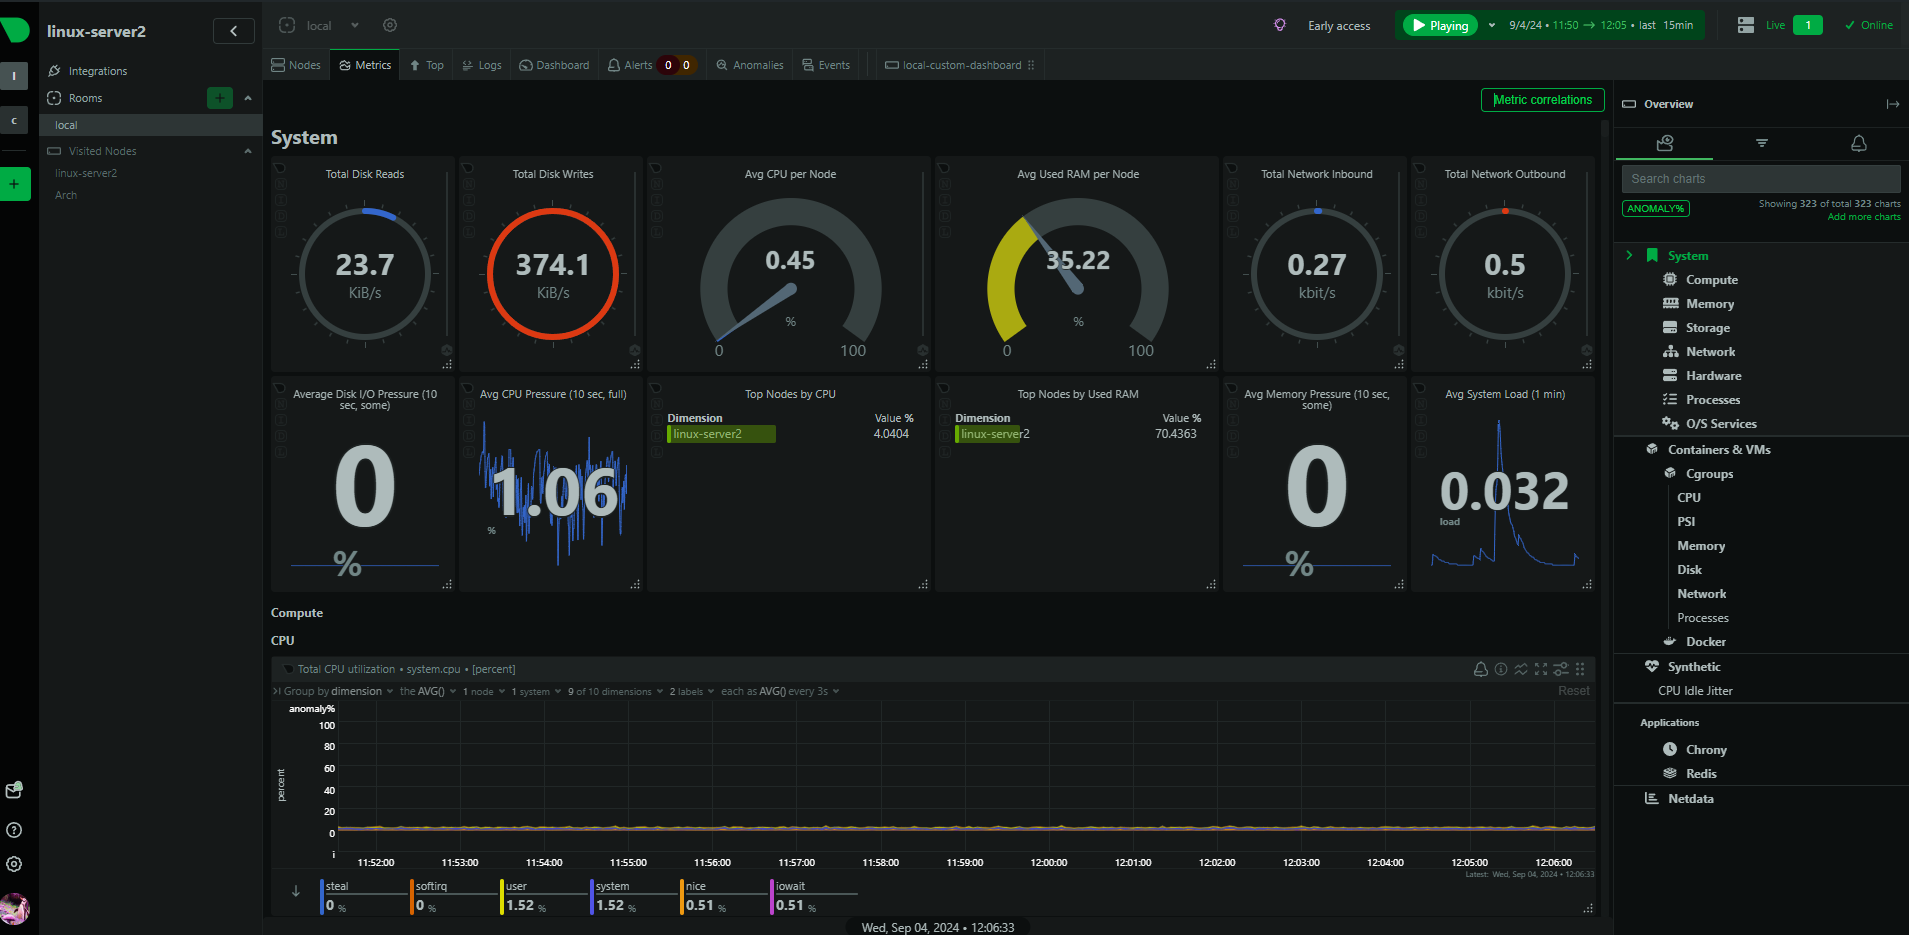
\includegraphics[width=1\textwidth]{Imatges/c-netdata.png}
\caption{Interfície visual de Netdata al servidor local} \end{figure}

\begin{figure}[!htbp] 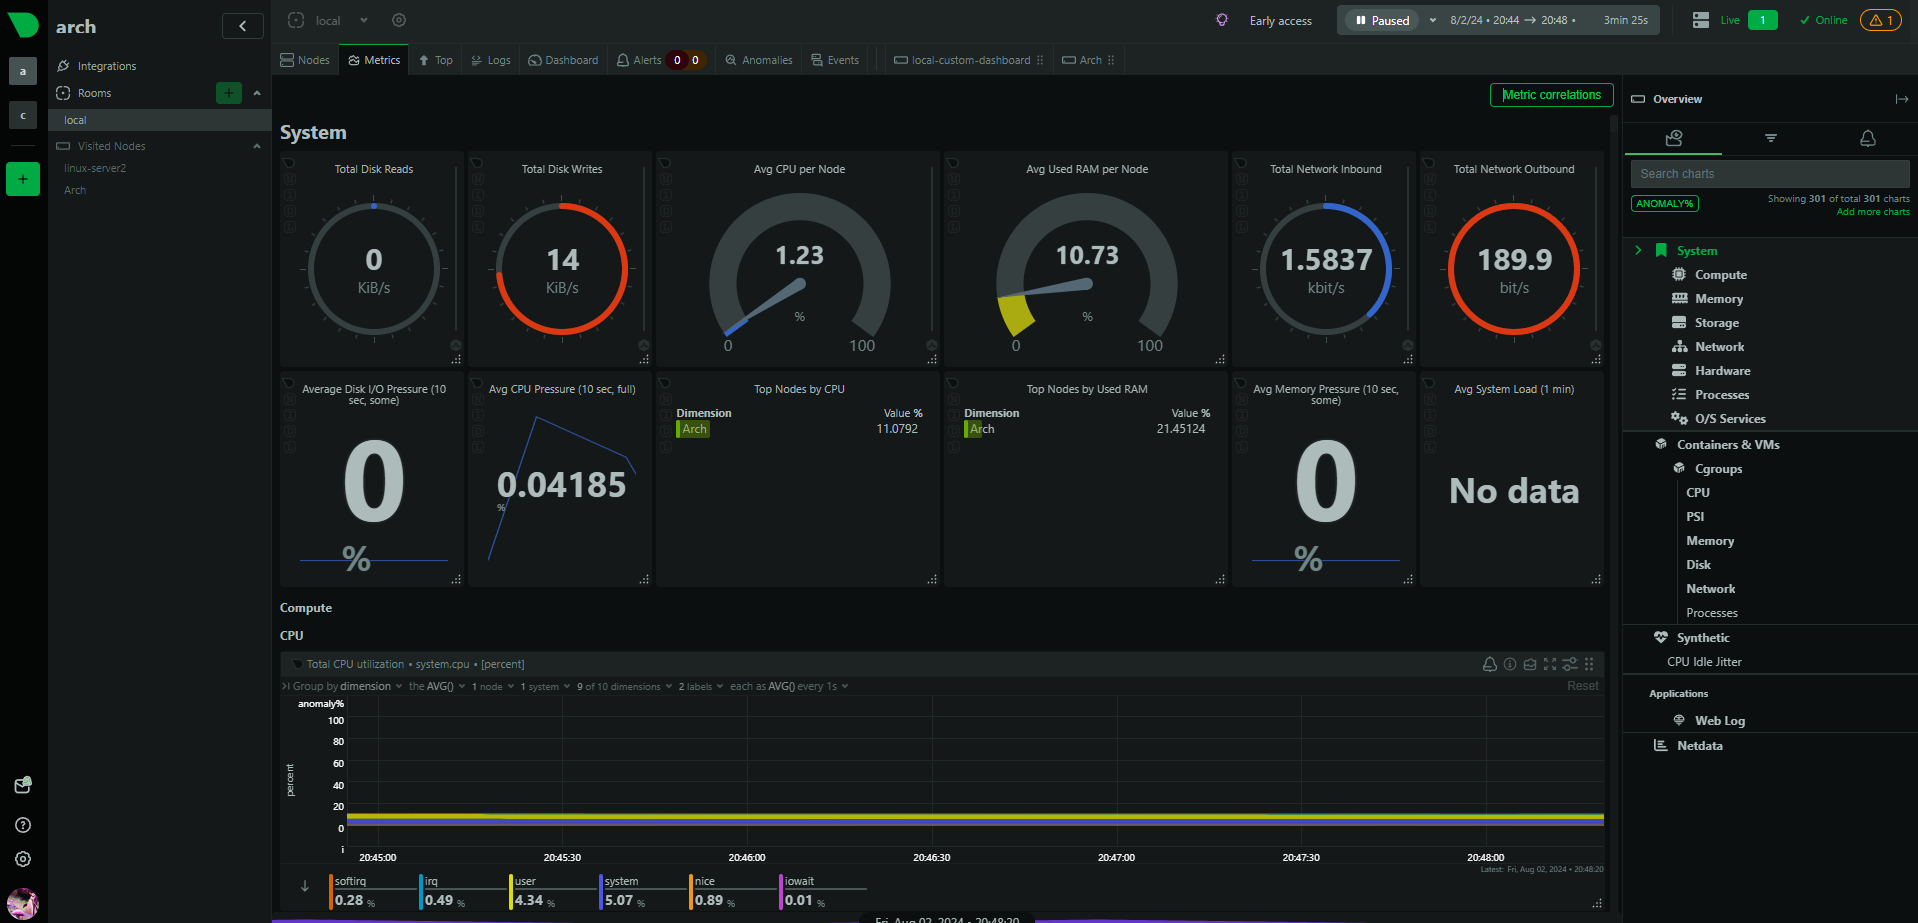
\includegraphics[width=1\textwidth]{Imatges/l-netdata.png}
\caption{Interfície visual de Netdata al servidor al núvol} \end{figure}

